\documentclass{article}

\usepackage[solutions]{../.template/xrcise}

\subject{Bio-inspired Artificial Intelligence}
\semester{Winter 2024}
\author{Leopold Lemmermann}

\begin{document}\createtitle


\sheet{Lecture Questions}
\begin{exercise}{Spiking Neural Networks}
  \begin{enumerate}
    \item Explain the concept of spiking neural networks and how they resemble biological information transmission.
    \item What is the difference between temporal coding and static learning?
    \item How is learning in spiking neural networks based on synaptic correlations?
    \item What is Spike-Timing-Dependent-Plasticity?
    \item Differentiate rate-coded, integrate-and-fire, and spike-response models.
  \end{enumerate}

  \begin{solution}
    \begin{enumerate}
      \item Spiking neural networks are a type of artificial neural network that model the behavior of biological neurons. They use spikes, or action potentials, to transmit information between neurons, similar to how biological neurons communicate.
      \item Temporal coding is a method of encoding information in the timing of spikes, while static learning is a method of encoding information in the strength of synaptic connections.
      \item Synaptic correlation describes the relationship between pre- and post-synaptic activity. This correlation is modeled using the weights of neural connections in spiking neural networks.
      \item Spike-Timing-Dependent-Plasticity (STDP) is a learning rule that strengthens or weakens synaptic connections based on the synaptic correlation.
      \item Rate-coded models use firing rates to encode information, only the frequency of spikes matters. Integrate-and-fire models integrate input signals over time and fire a spike when a threshold is reached, where leaky would describe the potential decay over time. Spike-response models model the response of a neuron to an input spike directly using a response function.
            \par Rate-coding is the simplest approach, integrate-and-fire provides a good trade-off between biological plausibility and computational efficiency, and spike-response models are more complex and biologically realistic.
    \end{enumerate}
  \end{solution}
\end{exercise}

\begin{exercise}{Computational Neural Networks}
  \begin{enumerate}
    \item Map these biological neural structures to artificial neural networks: neurons/synapses, action potentials, plasticity, and dopamine.
    \item Describe two different ANN architectures and their applications.
    \item What are some examples of useful applications of artificial neural networks?
  \end{enumerate}

  \begin{solution}
    \begin{enumerate}
      \item Neurons and synapses in biological neural structures correspond to nodes and weighted connections in artificial neural networks.
            \par Action potentials in biological neurons correspond to activation values in artificial neural networks.
            \par Plasticity in biological synapses describes the potential to change and corresponds to weight updates in backpropagation in artificial neural networks.
            \par Dopamine in biological reward systems corresponds to reward signals in artificial neural networks, like in reinforcement learning.
      \item Two different ANN architectures are convolutional networks, which are used for image processing tasks, and recurrent networks, which are used for sequential data processing tasks.
      \item Some examples of useful applications of artificial neural networks include speech and language processing, image recognition, and natural language understanding.
    \end{enumerate}
  \end{solution}
\end{exercise}

\begin{exercise}{Embodied Language Processing}
  \begin{enumerate}
    \item What models are suitable for explaining human natural language processing?
    \item Please explain Hebbian, SOM, and statistical learning.
    \item What is a grounded language?
    \item How can bio-inspired grounded language processing improve classic NLP methods?
  \end{enumerate}

  \begin{solution}
    \begin{enumerate}
      \item Models suitable for explaining human NLP include the Wernicke-Geschwind and the dual-stream model. The Wernicke-Geschwind model describes the language processing areas in the brain, while the dual-stream model describes the dorsal and ventral streams for speech perception and production.
      \item Hebbian learning is an unsupervised learning rule that strengthens synaptic connections between neurons that fire together. SOM learning is an unsupervised learning algorithm used in self-organizing maps to cluster similar input patterns into a topology map. Statistical learning is a method of learning from data by estimating the probability distribution of the data, and can be supervised or unsupervised.
      \item A grounded language is a language that is based on the physical world and is grounded in sensory-motor experiences.
      \item Bio-inspired grounded language processing can improve classic NLP methods by providing brain-inspired representations and mechanisms that better capture the structure and meaning of language.
    \end{enumerate}
  \end{solution}
\end{exercise}

\begin{exercise}{Robot Sound Localization}
  \begin{enumerate}
    \item Explain the concepts of ITD and ILD in a hybrid acoustic system.
    \item How can ITD and ILD be implemented in a hybrid spiking neural network?
  \end{enumerate}

  \begin{solution}
    \begin{enumerate}
      \item Interaural time difference (ITD) is the difference in time it takes for a sound to reach each ear, while interaural level difference (ILD) is the difference in intensity of a sound at each ear. In a hybrid acoustic system, ITD and ILD are used to localize sound sources in space.
      \item ITD is modeled by temporal delays in the input signals, and ILD is modeled by differences in the input amplitudes in a hybrid spiking neural network. These cues are combined to estimate the location of a sound source.
    \end{enumerate}
  \end{solution}
\end{exercise}

\begin{exercise}{Hierarchical Vision}
  \begin{enumerate}
    \item Which visual information is processed in which brain areas? % TODO: learn this
    \item What are the features filtered in the visual processing of the brain? % TODO: learn this
    \item Explain a hierarchical computational model for object recognition.
    \item How can deep learning be utilized for visual processing?
  \end{enumerate}

  \begin{solution}
    \begin{enumerate}
      \item V1 (Striate Cortex) for edge detection. V2 for texture. V3 for color and motion. V5 for motion and eye movements. (V2-5 Extrastriate Cortex). Ventral and dorsal streams for higher-level processing.
      \item The features filtered in the visual processing of the brain include edges, textures, shapes, and objects.
      \item A hierarchical computational model for object recognition involves multiple layers of processing, where each layer extracts increasingly complex features from the input data to recognize objects.
      \item Deep learning can be utilized for visual processing by using deep neural networks to learn hierarchical representations of visual data. These networks can automatically learn features from the data and perform tasks like object recognition and image classification.
    \end{enumerate}
  \end{solution}
\end{exercise}

\begin{exercise}{Crossmodal Processing}
  \begin{enumerate}
    \item Briefly explain one model for bio-inspired sound source localization, visual localization, and multisensory integration each.
    \item How effective are bio-inspired models in practice?
    \item Demonstrate similarities and differences between bio-inspired models and biological systems.
  \end{enumerate}

  \begin{solution}
    \begin{enumerate}
      \item One model for bio-inspired sound source localization is the duplex theory of sound localization, which uses interaural time difference (ITD) and interaural level difference (ILD) to localize sound sources. One model for bio-inspired visual localization is the hierarchical processing model, which uses multiple layers of processing to extract features from visual data. One model for bio-inspired multisensory integration is the Bayesian integration model, which combines information from multiple sensory modalities to make decisions.
      \item Bio-inspired models are effective in practice for tasks like sound source localization, visual localization, and multisensory integration. These models can capture the complexity and flexibility of biological systems and provide insights into how sensory information is processed in the brain.
      \item Bio-inspired models demonstrate behavioral and neurophysiological similarities with biological systems, such as the ability to localize sound sources, recognize objects, and integrate information from multiple sensory modalities. However, there are also differences between bio-inspired models and biological systems, such as the level of abstraction and complexity of the models.
    \end{enumerate}
  \end{solution}
\end{exercise}

\begin{exercise}{Behavior-based Robotics}
  \begin{enumerate}
    \item Explain the advantages of behavior-based robotics.
    \item How can behavior-based robotics be used for planning?
    \item What are the limits of behavior-based robotics?
  \end{enumerate}

  \begin{solution}
    \begin{enumerate}
      \item The advantages of behavior-based robotics include fast reaction times, robustness, the ability to follow multiple goals simultaneously, extensibility, simplicity, and computational tractability.
      \item Behavior-based robotics can be used for planning by combining simple behaviors to achieve complex goals. This approach allows robots to react to their environment in real-time and adapt to changing conditions.
      \item The limits of behavior-based robotics include the need for sufficient information from the local environment, the challenge of incorporating non-local information, the difficulty of learning global behavior, and the complexity of interactions in large-scale systems.
    \end{enumerate}
  \end{solution}
\end{exercise}

\begin{exercise}{Gesture recognition}
  \begin{enumerate}
    \item Explain the importance of gestures in communication and their role in multimodal systems.
    \item Which models are suitable for gesture recognition and how do they differ?
    \item How would you choose a model for gesture recognition?
  \end{enumerate}

  \begin{solution}
    \begin{enumerate}
      \item Gestures are an integral part of communication and play an important role in multimodal systems. They provide additional information beyond speech and can convey emotions, intentions, and context.
      \item Models suitable for gesture recognition include deep networks for feature extraction, recurrent networks like LSTM and GammaGWR for sequence modeling, and reservoir computing models for action selection. These models differ in their approach to feature extraction, sequence modeling, and action selection.
      \item When choosing a model for gesture recognition, it is important to consider the type of gestures being recognized, the complexity of the task, the amount of data available, and the computational resources required. Deep networks are suitable for feature extraction, recurrent networks are suitable for sequence modeling, and reservoir computing models are suitable for action selection.
    \end{enumerate}
  \end{solution}
\end{exercise}

\begin{exercise}{Evolutionary Computing}
  \begin{enumerate}
    \item Explain the advantages of evolutionary algorithms.
    \item What are the limits of evolutionary algorithms?
    \item Name and describe two evolutionary algorithms.
  \end{enumerate}

  \begin{solution}
    \begin{enumerate}
      \item The advantages of evolutionary algorithms include being a general heuristic for problem search, the ability to find good solutions in feasible computing time, and the possibility of distributed execution.
      \item The limits of evolutionary algorithms include the need for a large number of evaluations, the difficulty of tuning parameters, the risk of premature convergence, and the challenge of scaling to large problems.
      \item Two evolutionary algorithms are the genetic algorithm, which uses selection, crossover, and mutation operators to evolve a population of solutions, and ant colony optimization, which models the foraging behavior of ants to find optimal solutions to optimization problems.
    \end{enumerate}
  \end{solution}
\end{exercise}

\begin{exercise}{Neuro-Symbolic and Explainable AI Systems}
  \begin{enumerate}
    \item Explain the concept of neuro-symbolic systems and how they combine symbolic and connectionist AI.
    \item How can symbolic rules be extracted from neural networks?
    \item Describe different architectures for integrating symbolic and neural computing.
    \item How can images be processed by a neural network and visualized?
    \item Why are hybrid systems and explainable AI in the current focus of research?
  \end{enumerate}

  \begin{solution}
    \begin{enumerate}
      \item Neuro-symbolic systems combine symbolic and connectionist AI by integrating symbolic reasoning with neural network processing. These systems use symbolic rules to guide neural network learning and decision-making.
      \item Symbolic rules can be extracted from neural networks by analyzing the learned weights and activations of the network to identify patterns and rules that explain the network's behavior.
      \item Sequential architecture: neural network processing followed by (higher-level) symbolic reasoning. Embedding knowledge in neural networks: symbolic knowledge is encoded in the network's weights. Recurrent neural-symbolic models: continuous feedback between neural and symbolic processing. Knowledge-based NNs: symbolic rules are directly incorporated into the network architecture.
      \item Process images with CNN, visualize by analyzing the activations of the network, e.g., by using gradient-based methods to highlight important features.
      \item It is becoming increasingly important to explain AI systems and make their decisions transparent and interpretable. Hybrid systems combine the strengths of symbolic and neural computing to provide more robust and explainable AI solutions.
    \end{enumerate}
  \end{solution}
\end{exercise}

\begin{exercise}{Continual Learning for Robotic Action}
  \begin{enumerate}
    \item Explain the stability-plasticity dilemma and how it relates to continual learning.
    \item What is Hebbian learning?
    \item Outline the problem of catastrophic forgetting in neural networks and how it can be overcome.
    \item How could continual object recognition be approached?
    \item What are the applications of continual learning in natural language processing?
    \item Compare the state-of-the-art models with biological systems.
    \item How can continual learning be used to model higher-level cognitive functions in artificial systems?
  \end{enumerate}

  \begin{solution}
    \begin{enumerate}
      \item The stability-plasticity dilemma is the trade-off between the ability of a neural network to learn new information (plasticity) and the ability of the network to retain previously learned information (stability). Continual learning is the ability to incrementally learn over time without forgetting.
      \item Hebbian learning is a learning rule that strengthens synaptic connections between neurons that fire together.
      \item Catastrophic forgetting is the phenomenon where a neural network forgets previously learned information when learning new information. This problem can be overcome by using regularization, dynamic architectures, and rehearsal/replay.
      \item Continual object recognition can be approached by using self-organizing networks like Gamma-GWR to learn sequences of objects and by using hybrid models like Growing Dual-Memory (GDM) with memory replay to recognize objects over time.
      \item Applications of continual learning in natural language processing include continual language learning and open challenges in adapting to new tasks and data.
      \item State-of-the-art models are far from providing the flexibility, robustness, and scalability of biological systems. These models are limited in their ability to learn from new data and adapt to changing environments.
      \item Continual learning can be used to model higher-level cognitive functions in artificial systems by providing a framework for learning from new data, adapting to new tasks, and retaining previously learned information.
    \end{enumerate}
  \end{solution}
\end{exercise}


\sheet[2023]{1st exam}

\begin{exercise}{Multiple Choice}
  \begin{enumerate}
    \item The neighborhood in a self-organizing map (SOM) is computed as a
          \begin{itemize}
            \item Gaussian
            \item linear
            \item step
            \item constant
          \end{itemize}
          function of the distance between the winning neuron and the other neurons.

    \item A ground language is based on the
          \begin{itemize}
            \item ground truth.
            \item physical world.
            \item ground state.
            \item ground floor.
          \end{itemize}

    \item The ventriloquism effect is the illusion that a sound is coming from
          \begin{itemize}
            \item a different location
            \item the same Location
          \end{itemize}
          than the actual source.
  \end{enumerate}

  \begin{solution}
    \begin{enumerate}
      \item Gaussian.
      \item Physical world.
      \item A different location.
    \end{enumerate}
  \end{solution}
\end{exercise}

\begin{exercise}{General}
  \begin{enumerate}
    \item Explain the multisensory integration of different strength stimuli.
    \item What is the cocktail party effect?
  \end{enumerate}

  \begin{solution}
    \begin{enumerate}
      \item Multisensory integration is the process by which information from different sensory modalities is combined to form a unified perception. This process can enhance the detection and discrimination of stimuli and improve the accuracy and reliability of sensory processing.
      \item The cocktail party effect is the ability to focus on a single conversation in a noisy environment. This phenomenon allows individuals to selectively attend to one speaker while ignoring other competing sounds.
    \end{enumerate}
  \end{solution}
\end{exercise}

\begin{exercise}{Spiking Neural Networks}
  \begin{enumerate}
    \item Explain the difference between the leaky integrate-and-fire model and the integrate-and-fire model.
    \item Calculate the similarity angle between a weight vector $\mathbf{w} = [1, 2, 3]$ and an input vector $\mathbf{x} = [4, 5, 6]$.
    \item Compute the output of a perceptron with weights $\mathbf{w} = [1, 2, 3]$ and input $\mathbf{x} = [4, 5, 6]$.
  \end{enumerate}

  \begin{solution}
    \begin{enumerate}
      \item In the integrate-and-fire model, the neuron integrates input signals over time and fires a spike when the membrane potential reaches a threshold. In the leaky integrate-and-fire model, the neuron also integrates input signals over time, but the membrane potential decays over time in the absence of input. This leads to more realistic behavior and allows the neuron to adapt to changing input conditions.
      \item The similarity angle between two vectors $\mathbf{a}$ and $\mathbf{b}$ is given by
            \[ \theta = \arccos(\frac{\mathbf{a} \cdot \mathbf{b}}{\|\mathbf{a}\| \|\mathbf{b}\|}). \]
            For $\mathbf{w} = [1, 2, 3]$ and $\mathbf{x} = [4, 5, 6]$, we have
            \[ \cos(\theta) = \frac{1 \cdot 4 + 2 \cdot 5 + 3 \cdot 6}{\sqrt{1^2 + 2^2 + 3^2} \sqrt{4^2 + 5^2 + 6^2}} = \frac{32}{\sqrt{14} \sqrt{77}}. \]
      \item The output of a perceptron is given by
            \[
              y = \begin{cases}
                1 & \text{if } \mathbf{w} \cdot \mathbf{x} > 0, \\
                0 & \text{otherwise}.
              \end{cases}
            \]
            For $\mathbf{w} = [1, 2, 3]$, $\mathbf{x} = [4, 5, 6]$, and $b = 0$, we have
            \[
              y = \begin{cases}
                1 & \text{if } 1 \cdot 4 + 2 \cdot 5 + 3 \cdot 6 > 0, \\
                0 & \text{otherwise}.
              \end{cases}
            \]
    \end{enumerate}
  \end{solution}
\end{exercise}

\begin{exercise}{Visual Processing}
  \begin{enumerate}
    \item What do the different layers in a convolutional neural network (CNN) learn?
    \item Compute the filtering in a CNN layer with a $5 \times 5$ matrix and a $3 \times 3$ filter, stride $1$, and no padding.
    \item Draw a diagram of the orientation and firing rate of a simple cell for a line of different orientations.
  \end{enumerate}

  \begin{solution}
    \begin{enumerate}
      \item The different layers in a CNN learn different features of the input data. The first layers typically learn low-level features like edges and textures, while later layers learn higher-level features like shapes and objects.
      \item The filtering in a CNN layer with a $5 \times 5$ matrix and a $3 \times 3$ filter, stride $1$, and no padding can be computed by sliding the filter over the input matrix and computing the dot product at each position. The resulting output will be a $3 \times 3$ matrix.
      \item The orientation and firing rate of a simple cell for a line of different orientations can be visualized in a diagram with the orientation on the $x$-axis and the firing rate on the $y$-axis. It's a normal distribution from -90° to +90° with the peak firing rate at 0°.
    \end{enumerate}
  \end{solution}
\end{exercise}

\begin{exercise}{Audio Processing}
  Explain interaural time difference (ITD) and interaural level difference (ILD) and which one is used for high and low frequencies.

  \begin{solution}
    Interaural time difference (ITD) is the difference in time it takes for a sound to reach each ear, while interaural level difference (ILD) is the difference in intensity of a sound at each ear. ITD is used for low frequencies, while ILD is used for high frequencies.
  \end{solution}
\end{exercise}

\begin{exercise}{Behavior}
  \begin{enumerate}
    \item Explain a Braitenberg vehicle with an example and name the behavior of your example vehicle.
    \item Complete the flow chart of the functional decomposition of the classical approach for a robot controller:
          \begin{center}sensors $\rightarrow$ \_ $\rightarrow$ \_ $\rightarrow$ \_ $\rightarrow$ \_ $\rightarrow$ actuators.\end{center}
    \item Explain the advantage of a behavior-based approach to robotics.
  \end{enumerate}

  \begin{solution}
    \begin{enumerate}
      \item A Braitenberg vehicle is a simple robot that exhibits complex behavior through the direct coupling of sensors to actuators. An example of a Braitenberg vehicle is a light-seeking robot that moves towards a light source. The behavior of this example vehicle is phototaxis.
      \item The flow chart of the functional decomposition of the classical approach for a robot controller is: sensors $\rightarrow$ perception $\rightarrow$ modeling $\rightarrow$ planning $\rightarrow$ execution $\rightarrow$ actuators.
      \item The advantage of a behavior-based approach to robotics is that it allows for the development of complex behaviors through the combination of simple behaviors. This approach is more robust and adaptable to changing environments than traditional control architectures.
    \end{enumerate}
  \end{solution}
\end{exercise}

\begin{exercise}{Evolutionary Computing}
  \begin{figure}[H]
  \centering
  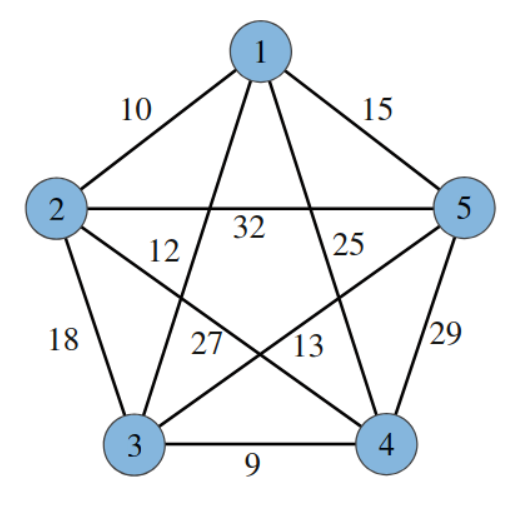
\includegraphics[width=.4\textwidth]{res/tsp.png}
  \caption{The TSP problem}\label{fig:tsp}
\end{figure}

  \begin{enumerate}
    \item Draw a cycle graph with the nearest-neighbor heuristic for the traveling salesman problem.
    \item Find the shortest distance between city $1$ and city $4$ in the graph.
    \item Describe a recombination and mutation algorithm for the example you provided.
    \item Explain optimization strategies for this algorithm.
  \end{enumerate}

  \begin{solution}
    \begin{enumerate}
      \item A cycle graph with arrow labels is a graph where each node is connected to the next node in a cycle, and the arrows indicate the direction of the cycle.
      \item The shortest distance between city $1$ and city $4$ in the graph is $1\to3\to4$.
      \item An approach to solving the traveling salesman problem using recombination and mutation could involve combining the paths of two solutions to create a new solution and randomly swapping cities in the solution to introduce diversity.
      \item Optimization strategies for this algorithm could include using a genetic algorithm to evolve a population of solutions, using local search to improve the quality of solutions, and using elitism to preserve the best solutions.
    \end{enumerate}
  \end{solution}
\end{exercise}



\sheet[2022]{1st exam}

\begin{exercise}{Multiple Choice}
  \begin{enumerate}
    \item In
          \begin{itemize}
            \item Multilayer perceptrons (MLP)
            \item Convolutional neural networks (CNN)
            \item Self-organizing maps (SOM)
            \item none of the above
          \end{itemize}
          is backpropagation used for learning.

    \item An embodied language is based on
          \begin{itemize}
            \item the physical world.
            \item ground truth.
            \item ground state.
            \item ground floor.
          \end{itemize}

    \item What are the two streams and their tasks in human vision?
          \begin{itemize}
            \item Dorsal stream for spatial vision and ventral stream for object recognition
            \item Ventral stream for spatial vision and dorsal stream for object recognition
          \end{itemize}
  \end{enumerate}

  \begin{solution}
    \begin{enumerate}
      \item Multilayer perceptron (MLP)
      \item Language is based on the physical world.
      \item Dorsal stream for spatial vision and ventral stream for object recognition
    \end{enumerate}
  \end{solution}
\end{exercise}

\begin{exercise}{Attention}
  \begin{enumerate}
    \item Name and explain three ways to measure the attention of a human.
    \item Describe two models to measure or visualize human attention.
    \item Name advantages and disadvantages of the two models you proposed.
  \end{enumerate}

  \begin{solution}
    \begin{enumerate}
      \item Three ways to measure the attention of a human are eye tracking, reaction time, and brain imaging.
      \item Two models to measure or visualize human attention are the spotlight model and the zoom lens model.
      \item The spotlight model has the advantage of being simple and intuitive, but it has the disadvantage of oversimplifying the attentional process. The zoom lens model has the advantage of being more flexible and dynamic, but it has the disadvantage of being more complex and difficult to interpret.
    \end{enumerate}
  \end{solution}
\end{exercise}

\begin{exercise}{Vision}
  \begin{enumerate}
    \item Name the two streams and their task that are present in human vision.
    \item Explain rods and cones.
    \item Explain the similarity between a convolutional neural network with convolution and max pooling layers and the visual cortex.
    \item Visualize the firing rate of a simple cell for a line of different orientation in a diagram with the orientation on the $x$-axis and the firing rate on the $y$-axis.
    \item Given a $5 \times 5$ matrix and a $3 \times 3$ filter, compute the convolution (no padding, stride $1$).
  \end{enumerate}

  \begin{solution}
    \begin{enumerate}
      \item The two streams present in human vision are the dorsal stream for spatial vision and the ventral stream for object recognition.
      \item Rods and cones are photoreceptor cells in the retina that are responsible for detecting light. Rods are sensitive to low light levels and are responsible for night vision, while cones are sensitive to color and are responsible for daylight vision.
      \item A convolutional neural network with convolution and max pooling layers is similar to the visual cortex in that both systems use hierarchical processing to extract features from the input data.
      \item The firing rate of a simple cell for a line of different orientations can be visualized in a diagram with the orientation on the $x$-axis and the firing rate on the $y$-axis.
      \item Given a $5 \times 5$ matrix and a $3 \times 3$ filter, the convolution (no padding, stride $1$) can be computed by sliding the filter over the input matrix and computing the dot product at each position. The resulting output will be a $3 \times 3$ matrix.
    \end{enumerate}
  \end{solution}
\end{exercise}

\begin{exercise}{Sound Localization}
  \begin{enumerate}
    \item Compute the cross-correlation steps on two signals until the maximum cross-correlation value is reached.
    \item Name and explain the two cues used to perform sound localization. Which one works best for high/low frequencies?
  \end{enumerate}

  \begin{solution}
    \begin{enumerate}
      \item The cross-correlation steps on two signals can be computed by sliding one signal over the other and computing the dot product at each position until the maximum cross-correlation value is reached.
      \item The two cues used to perform sound localization are interaural time difference (ITD) and interaural level difference (ILD). ITD works best for low frequencies, while ILD works best for high frequencies.
    \end{enumerate}
  \end{solution}
\end{exercise}

\begin{exercise}{Behavior}
  \begin{enumerate}
    \item Explain a Braitenberg vehicle with an example and name the behavior of your example vehicle.
    \item Complete the flow chart of the functional decomposition of the classical approach for a robot controller: sensors $\rightarrow$ blank $\rightarrow$ blank $\rightarrow$ blank $\rightarrow$ blank $\rightarrow$ actuators.
  \end{enumerate}

  \begin{solution}
    \begin{enumerate}
      \item A Braitenberg vehicle is a simple robot that exhibits complex behavior through the direct coupling of sensors to actuators. An example of a Braitenberg vehicle is a light-seeking robot that moves towards a light source. The behavior of this example vehicle is phototaxis.
      \item The flow chart of the functional decomposition of the classical approach for a robot controller is: sensors $\rightarrow$ perception $\rightarrow$ cognition $\rightarrow$ planning $\rightarrow$ control $\rightarrow$ actuators.
    \end{enumerate}
  \end{solution}
\end{exercise}

\begin{exercise}{Continual Learning}
  \begin{enumerate}
    \item Explain the stability-plasticity dilemma.
    \item Explain catastrophic forgetting and a model where this effect could arise.
    \item Name and describe two strategies of continual learning.
  \end{enumerate}

  \begin{solution}
    \begin{enumerate}
      \item The stability-plasticity dilemma is the trade-off between the ability of a neural network to learn new information (plasticity) and the ability of the network to retain previously learned information (stability).
      \item Catastrophic forgetting is the phenomenon where a neural network forgets previously learned information when learning new information. This effect could arise in a model where the network is trained on a sequence of tasks without preserving the knowledge learned on previous tasks.
      \item Two strategies of continual learning are rehearsal, where the network is periodically trained on previously learned tasks, and regularization, where the network is penalized for changing its weights too much.
    \end{enumerate}
  \end{solution}
\end{exercise}

\begin{exercise}{Language Processing}
  \begin{enumerate}
    \item Name the two streams important in language processing and their tasks.
    \item Describe CBOW (Continuous Bag-of-word) and Skip-gram.
    \item Describe the difference between the earlier Wernicke's model and the later Pulvermüller's model.
  \end{enumerate}

  \begin{solution}
    \begin{enumerate}
      \item The two streams important in language processing are the dorsal stream for speech perception and the ventral stream for speech production.
      \item CBOW (Continuous Bag-of-word) and Skip-gram are two models used for word embedding in natural language processing. CBOW predicts a target word from its context, while Skip-gram predicts the context words from a target word.
      \item The difference between the earlier Wernicke's model and the later Pulvermüller's model is that Wernicke's model is based on a sequential processing model of language, while Pulvermüller's model is based on a distributed processing model of language.
    \end{enumerate}
  \end{solution}
\end{exercise}

\begin{exercise}{Computational Neural Networks}
  \begin{enumerate}
    \item Explain three steps of the backpropagation algorithm and explain the termination criteria.
    \item Name and shortly describe the three fundamental ANN learning paradigms.
    \item Explain how the learning rate parameter could be chosen.
  \end{enumerate}

  \begin{solution}
    \begin{enumerate}
      \item Three steps of the backpropagation algorithm are forward propagation, backward propagation, and weight update. The termination criteria for backpropagation is typically based on the convergence of the loss function.
      \item The three fundamental ANN learning paradigms are supervised learning, unsupervised learning, and reinforcement learning. Supervised learning involves learning from labeled data, unsupervised learning involves learning from unlabeled data, and reinforcement learning involves learning from rewards and punishments.
      \item The learning rate parameter could be chosen using a grid search or random search over a range of values, or by using adaptive learning rate methods like AdaGrad or Adam.
    \end{enumerate}
  \end{solution}
\end{exercise}

\end{document}